% =====================================================================
%  第四部分  如何确认结果正确
% =====================================================================
\part{如何确认结果正确}

程序能跑出数字，不等于数字是对的。
这一部分讲怎么判断结果可不可信，
以及结果里那些数字分别说明什么。

% =====================================================================
\section{为什么必须验证}

\subsection{程序不会告诉你它算错了}

这是初学者最容易踩的坑。如果代码里公式写错了，
程序不会报错，它会照常运行，
然后给出一个看起来完全正常的数字。

举一个具体的例子。假设在写表面边界条件时，
把传质系数的系数写成了 $\dfrac{1}{4}h_mR$ 而不是 $\dfrac{1}{2}h_mR$。
程序照样能跑，曲线照样光滑，
但表面的干燥速度会慢一半，最后的烘干时间会明显偏长。
从输出上看不出任何异常。

再举一个例子。假设数组的索引搞错了，
把温度的最后一个分量当成水分来用。
程序也不会报错，但结果完全没有意义。

\why{为什么这类错误难以发现}
因为数值方法本身就是在做近似，
输出总是带着一点误差。
当误差的来源既有正常的离散误差又有真正的代码错误时，
两者混在一起，从数字上分不清。

唯一的解决办法是：拿一个已知正确答案的问题去检验程序。
如果程序在已知答案的问题上给出正确答案，
那么在未知答案的问题上给出正确答案的可能性就大得多。

\keypoint
验证不是可选项，是必需项。
没有验证过的程序，输出的数字不能写进论文。

\subsection{验证的层次}

本文用了三层验证，一层比一层强。

\begin{center}
\begin{tabular}{@{}clp{7.6cm}@{}}
\toprule
层次 & 名称 & 做法 \\
\midrule
一 & 与精确解比较 & 找一个有公式解的问题，看程序算得对不对 \\
二 & 网格加密 & 把节点数加倍，看结果是否收敛到同一个值 \\
三 & 多方法互证 & 用完全不同的方法算同一个问题，看结果是否一致 \\
\bottomrule
\end{tabular}
\end{center}

下面三章分别讲这三种。

% =====================================================================
\section{第一层验证：与精确解比较}

\subsection{精确解从哪里来}

问题一的温度场有精确解，就是第三部分第十三章讲的贝塞尔--杜阿梅尔展开式。

要特别说明的是，这个精确解不是随便找的，
它是在完全相同的方程、完全相同的边界条件、
完全相同的初值下推导出来的。
所以它可以作为程序的标准答案。

\subsection{比较的方法}

具体做法是：把 $N=64$ 的谱解和精确解在
从圆心到表面的 $201$ 个位置上逐点相减，取差值的绝对值最大的那个。

结果如表~\ref{tab:verify1}。

\begin{table}[H]
\centering
\small
\caption{谱解与精确解的偏差（问题一温度场，$t=1800$ 秒）}
\label{tab:verify1}
\begin{tabular}{@{}lcccccc@{}}
\toprule
节点数 $N$ & 4 & 6 & 8 & 16 & 32 & 64 \\
\midrule
最大偏差 / 开尔文 & $7.59\times10^{-6}$ & $2.88\times10^{-10}$ & $1.09\times10^{-10}$
& $1.13\times10^{-10}$ & $1.14\times10^{-10}$ & $1.14\times10^{-10}$ \\
\bottomrule
\end{tabular}
\end{table}

\subsection{怎么读这张表}

先看最左边两格。$N=4$ 时的偏差是 $7.59\times10^{-6}$ 开尔文，
$N=6$ 时降到 $2.88\times10^{-10}$ 开尔文。
节点数从 $4$ 加到 $6$，只多了两个节点，偏差掉了四个多数量级。
这是谱收敛的典型表现：精度不是慢慢爬升，而是跳台阶。

再看右边几格。从 $N=8$ 开始，偏差稳定在 $1.1\times10^{-10}$ 附近，
$N$ 继续加到 $64$ 也不再下降。

这个不再下降的现象需要解释清楚，否则会被误读成方法失效。
它说明偏差已经不再是空间离散造成的，而是时间积分造成的。
判断依据是下面这组数据：把时间相对容差收紧，
偏差跟着一起变，而空间节点数不变。

\begin{center}
\begin{tabular}{@{}lc@{}}
\toprule
时间相对容差 & 偏差 / 开尔文 \\
\midrule
$10^{-8}$ & $1.03\times10^{-7}$ \\
$10^{-10}$ & $2.34\times10^{-9}$ \\
$10^{-12}$ & $1.14\times10^{-10}$ \\
\bottomrule
\end{tabular}
\end{center}

容差每收紧两个数量级，偏差就下降一个多数量级，两者同步变化。
所以 $1.1\times10^{-10}$ 这个平台是时间容差 $10^{-12}$ 决定的，
不是计算机能表示的极限。
双精度浮点数在温度 $34$ 附近的表示间隔约为 $10^{-14}$ 开尔文，
比这个平台还小四个数量级。

\why{这说明什么}
说明空间离散的误差已经小到看不见了。
换句话说，只用 $7$ 个点，空间精度就已经落在时间精度的水平以下。

如果在 $N=8$ 的时候偏差还很大，
或者偏差随 $N$ 增大而缓慢下降，
那就说明空间离散有问题，需要检查微分矩阵或者边界条件的写法。

\subsection{这个 10 的负 10 次方意味着什么}

温度的量级是几十摄氏度。
偏差是 $10^{-10}$ 开尔文，
相当于把温度算准到小数点后十位。

作为对比，工程上一般认为小数点后四位就够了。
所以这个精度远远超过需要。

\keypoint
与精确解比较的结果是：偏差约 $10^{-10}$，
而且这个偏差由时间容差控制，不是空间离散造成。
这证明空间离散与边界条件的实现是正确的。

% =====================================================================
\section{第二层验证：网格加密看收敛}

\subsection{收敛是什么意思}

数值方法用一个有限的网格去近似连续的区域。
网格越密，近似越好。
当网格无限加密时，数值解应该趋近于真实的连续解。
这个性质叫收敛。

如果程序写错了，加密网格往往不会让它收敛到正确答案，
而是收敛到某个错误的值，或者干脆发散。

所以做法是：用一系列越来越密的网格各算一次，
看结果是否稳定下来。

\begin{figure}[H]
\centering
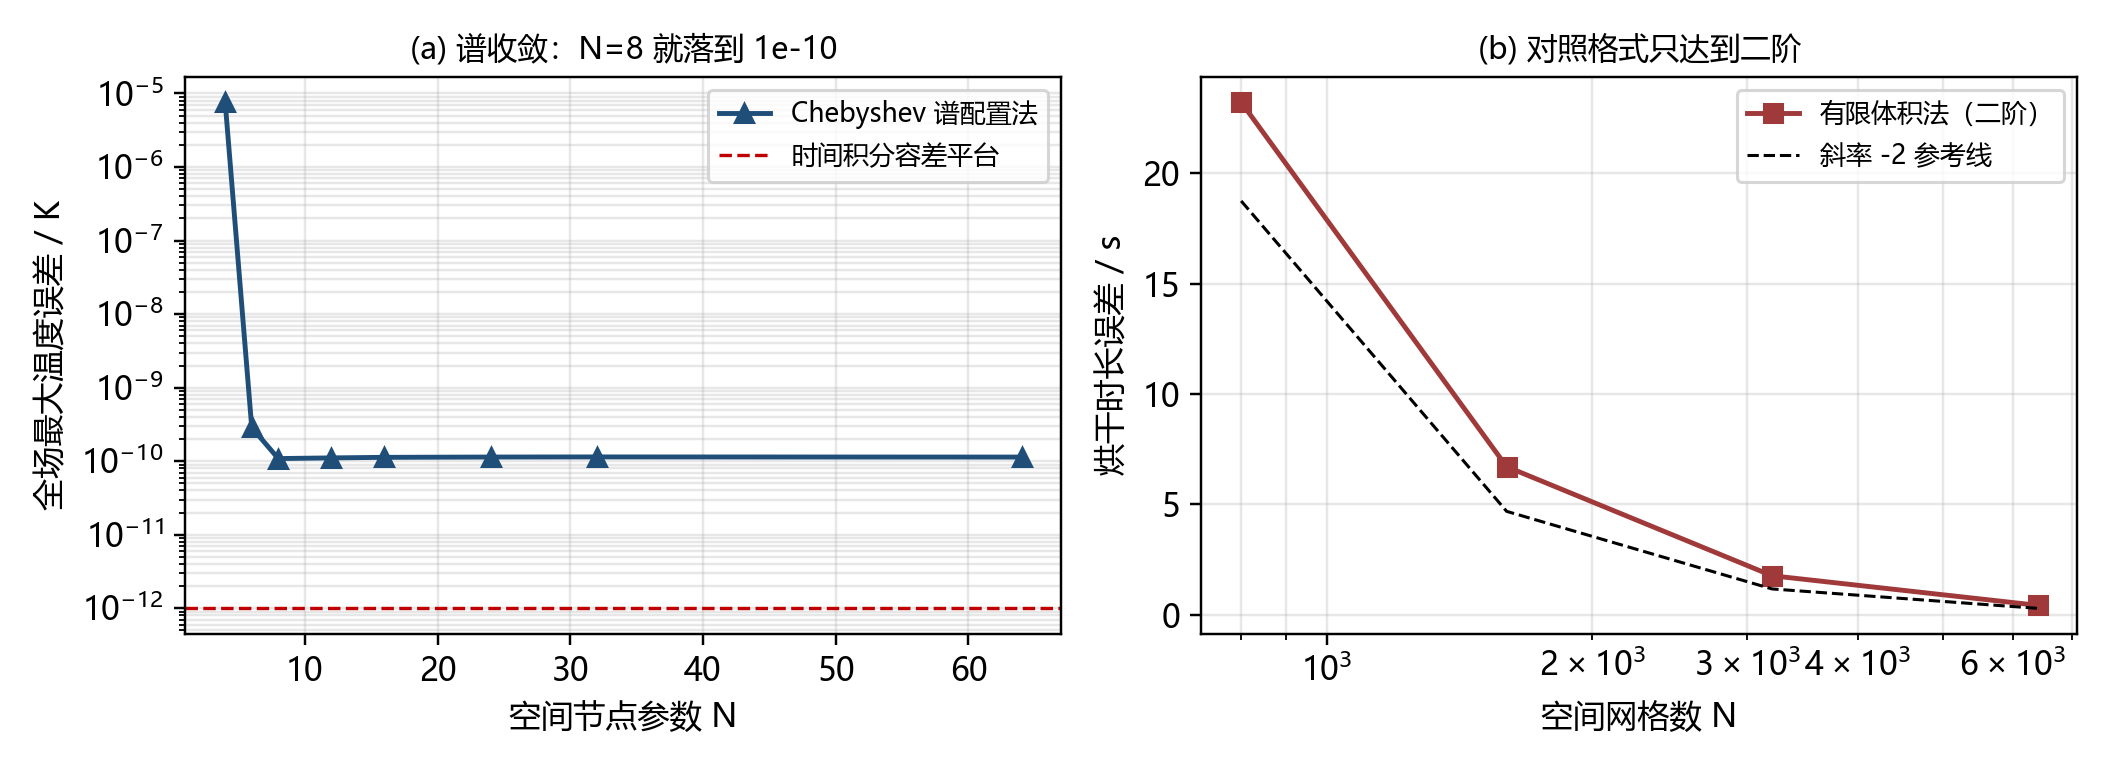
\includegraphics[width=0.96\textwidth]{fig/fig_conv.png}
\caption{两种离散方式的空间收敛。(a) 谱配置法：节点参数 N 从 4 增到 6 时误差从 7.6e-6 掉到 2.9e-10，此后落在时间积分容差平台上不再下降；(b) 有限体积对照格式只达到二阶收敛。}
\label{fig:conv}
\end{figure}

\subsection{空间方向的加密}

对问题三的烘干时间做这个实验。节点数从 $24$ 增加到 $128$，
每一步算出的烘干时间如表~\ref{tab:verify2}。

\begin{table}[H]
\centering
\small
\caption{烘干时间随节点数的变化（问题三）}
\label{tab:verify2}
\begin{tabular}{@{}lcccccc@{}}
\toprule
节点数 $N$ & 24 & 32 & 48 & 64 & 96 & 128 \\
\midrule
烘干时间 / 秒 & 205557.9 & 205565.2 & 205572.3 & 205574.5 & 205575.4 & 205575.5 \\
相邻变化 / 秒 & --- & $+7.3$ & $+7.1$ & $+2.2$ & $+0.9$ & $+0.1$ \\
\bottomrule
\end{tabular}
\end{table}

\subsection{怎么读这张表}

看最后一行的相邻变化。从 $7.3$ 秒降到 $7.1$ 秒，
再降到 $2.2$ 秒、$0.9$ 秒、最后 $0.1$ 秒。
变化量在持续减小。

当 $N$ 从 $96$ 增加到 $128$ 时，结果只变了 $0.1$ 秒。
这说明再继续加密，结果也不会明显变化了。

本文最终采用的是 $N=64$ 的生产值 $205574.5$ 秒，
因为交付的结果文件 result3.xlsx 就是按这个设置写出的。
$N=128$ 给出 $205575.5$ 秒，两者相差 $1.0$ 秒，
相对于五十七小时是万分之零点零五，可以忽略。

\why{这个衰减速度说明了什么}
这里的衰减是谱方法的典型特征，也就是衰减得非常快。
如果换成普通的差分方法，同样的节点数范围内，
变化量会缓慢地按平方反比下降，
需要上千个节点才能达到这个稳定程度。

\subsection{时间方向的加密}

用另一种格式，也就是第三部分提到的节点中心有限体积加定步长方法，
做一次时间步长的实验。结果如表~\ref{tab:verify3}。

\begin{table}[H]
\centering
\small
\caption{烘干时间随时间步长的变化，对照格式，节点数 $1600$}
\label{tab:verify3}
\begin{tabular}{@{}lccccc@{}}
\toprule
时间步 $\Delta t$ / 秒 & 10 & 5 & 2 & 1 & 0.5 \\
\midrule
烘干时间 / 秒 & 205553.80 & 205561.35 & 205565.88 & 205567.39 & 205568.10 \\
相邻变化 / 秒 & --- & $+7.55$ & $+4.53$ & $+1.51$ & $+0.71$ \\
\bottomrule
\end{tabular}
\end{table}

这张表的读法和上一张完全不同。

步长从 $2$ 秒减到 $1$ 秒，烘干时间增加 $1.51$ 秒。
再从 $1$ 秒减到 $0.5$ 秒，增加 $0.71$ 秒。
后一个增量大约是前一个的一半。

每把步长减半，变化量也减半。
这是误差与步长成正比的特征，专业上叫做一阶收敛。
对比上一张表，谱方法在空间上是跳跃式收敛，
而这个格式在时间上只能按倍数慢慢逼近。

\why{一阶收敛说明什么}
说明这个格式的时间误差与步长成正比，减小得很慢。
要把时间误差从秒的量级压到零点几秒，步长必须一直减下去，
而且每减一半只能换来一半的改善。

这也说明，如果在干燥后期把步长放宽到 $10$ 秒，
算出来的烘干时间是 $205553.8$ 秒，
比生产值 $205574.5$ 秒小了 $20.7$ 秒。
这个偏差只占万分之一点零，
但在比较不同来源的烘干时长时足以造成困扰。

\keypoint
网格加密实验告诉我们两件事。
第一，本文主求解器的空间收敛很快，$N$ 到 $64$ 以后结果就稳定了。
第二，对照格式在时间方向只有一阶精度，
如果步长放得太宽会带来十几秒的系统偏差。

% =====================================================================
\section{第三层验证：多种方法互证}

\subsection{为什么要用不同方法}

前两层验证都还在自己的体系内。
与精确解比较用到了精确解，
网格加密看的是自己的收敛行为。

第三层验证更强：用完全不同的离散思想去解同一组方程。
如果两种毫不相干的方法给出同一个答案，
那么两者同时出错的概率极低。

本文用了三种方法。

\begin{center}
\begin{tabular}{@{}clp{7.4cm}@{}}
\toprule
代号 & 方法 & 特征 \\
\midrule
甲 & 闭式解 & 用贝塞尔函数级数，没有离散网格 \\
乙 & 谱配置法 & 切比雪夫节点，全局耦合，谱精度 \\
丙 & 守恒型有限体积 & 均匀网格，只用到相邻点，空间二阶，
时间用等步长后向欧拉，靠步长趋于零的外推消掉时间误差 \\
\bottomrule
\end{tabular}
\end{center}

三种方法的数学基础完全不同。甲是解析的，
乙用的是全局多项式，丙用的是局部守恒。

\subsection{比较结果}

\begin{table}[H]
\centering
\small
\caption{三种方法的比较（问题一）}
\begin{tabular}{@{}lccc@{}}
\toprule
量 & 甲：闭式解 & 乙：谱配置法 & 丙：有限体积 \\
\midrule
$T(0,1800)$ / 摄氏度 & 34.0424989 & 34.042499 & --- \\
$T(R_0,1800)$ / 摄氏度 & 37.1989220 & 37.198922 & 37.1989221 \\
$C(R_0,1800)$ / (kg/kg) & --- & 1.51091810 & 1.51092243 \\
$C(R_0,1200)$ / (kg/kg) & --- & 1.65914239 & 1.65915047 \\
\bottomrule
\end{tabular}
\end{table}

\subsection{怎么读这张表}

先说丙列的来历，这一点必须交代清楚，否则数字无法复核。
丙这一列不是直接算出来的一个数，而是这样得到的：
在网格数 $N=400$ 下取两个时间步 $0.5$ 秒与 $0.25$ 秒各算一次，
再用后向欧拉的一阶格式做一次步长趋于零的外推，
公式是外推值等于半步长的值减去两者之差。
复跑报告的第六节列出了这两次计算的全部原始数据，
用计算器就能复核上表里丙列的三个数。

第一行丙列留空，原因是复跑报告第六节的对照输出里没有圆心温度，
这里不给出没有出处的数字。

再看数值本身。甲与乙在温度上的差别是最后一位小数，
数量级是 $10^{-7}$。乙与丙在表面温度上吻合到
$7\times10^{-8}$ 开尔文。

对于水分，因为没有闭式解，只能比较乙和丙。
在 $C(R_0,1800)$ 这一格，两者分别是
$1.51091810$ 与 $1.51092243$，差别是 $4.3\times10^{-6}$。
在 $C(R_0,1200)$ 这一格，两者分别是
$1.65914239$ 与 $1.65915047$，差别是 $8.1\times10^{-6}$。

把这三个量四舍五入到四位小数：
表面温度三法都是 $37.1989$，
表面水分在 $1800$ 秒三法都是 $1.5109$，
表面水分在 $1200$ 秒乙给出 $1.6591$、丙给出 $1.6592$，差在第四位小数。
交付文件统一保留四位小数，所以前两项三法一致，
第三项在第四位小数上有一格之差。

\why{有限体积的结果为什么不是恰好相等}
因为它只做到空间二阶，本身带有离散误差，
而且在 $N=400$ 时空间误差还没有被外推掉。
上表里丙的值已经把时间误差消掉，剩下的就是这部分空间误差，
量级在 $10^{-6}$ 到 $10^{-5}$。
两种方法都收敛到同一个连续解，只是在有限网格下各自带着不同的小误差。

\subsection{一次特别的比较}

除了上面这三种，本文还和第四种格式比过一次。
在问题二的早期时刻，$0.5$ 小时、圆心处：

\begin{center}
\begin{tabular}{@{}lc@{}}
\toprule
方法 & 温度 / 摄氏度 \\
\midrule
谱配置法，节点数 $N=64$ 至 $128$ & 32.565670279 \\
节点中心有限体积加定步长方法 & 32.565670347 \\
\midrule
差值 & $6.8\times10^{-8}$ \\
\bottomrule
\end{tabular}
\end{center}

第二种方法的值是把它的一阶时间误差扣掉以后得到的。
两种完全不同的离散格式在连续极限上吻合到 $10^{-8}$ 的量级，
这是一个很强的证据。

\keypoint
三种方法的互证结果是：在四位小数的精度上完全一致。
这排除了代码存在系统性错误的可能。

% =====================================================================
\section{灵敏度分析结果怎么读}

\subsection{做了什么事}

把某个参数乘上一个系数，重新算一遍烘干时间，
看结果变化多少。做了十二组。

\subsection{结果}

\begin{table}[H]
\centering
\small
\caption{参数扰动对烘干时间的影响（基准值 205574.519 秒）}
\begin{tabular}{@{}lccc@{}}
\toprule
扰动的参数 & 烘干时间 / 秒 & 相对变化 & 排名 \\
\midrule
活化温度 $E$ 加百分之二 & 254624.0 & $+23.86\%$ & 1 \\
活化温度 $E$ 减百分之二 & 167355.9 & $-18.59\%$ & 2 \\
活化浓度指数 $a$ 加百分之二 & 215664.2 & $+4.91\%$ & 3 \\
活化浓度指数 $a$ 减百分之二 & 196057.7 & $-4.63\%$ & 4 \\
扩散系数前因子 $D_0$ 减百分之二 & 209277.8 & $+1.80\%$ & 5 \\
扩散系数前因子 $D_0$ 加百分之二 & 202019.9 & $-1.73\%$ & 6 \\
烘房设定温度减 $0.2$ 度 & 206911.0 & $+0.65\%$ & 7 \\
烘房设定温度加 $0.2$ 度 & 204250.0 & $-0.64\%$ & 8 \\
传质系数 $h_m$ 减百分之二 & 206055.5 & $+0.23\%$ & 9 \\
传质系数 $h_m$ 加百分之二 & 205116.3 & $-0.22\%$ & 10 \\
换热系数 $h$ 减百分之二 & 205580.3 & $+0.003\%$ & 11 \\
换热系数 $h$ 加百分之二 & 205568.9 & $-0.003\%$ & 12 \\
\bottomrule
\end{tabular}
\end{table}

\subsection{三个要读懂的地方}

第一，活化温度的影响最大，而且方向相反的两个扰动幅度不同。
加百分之二带来 $+23.86\%$，减百分之二带来 $-18.59\%$。
不对称的原因是这个参数出现在指数上，
指数函数不是线性的，向上和向下的效果自然不一样。

第二，换热系数几乎没影响，不到万分之一。
这个结果一开始可能让人意外，因为直觉上觉得换热快干燥就快。
解释是这样的：温度在两个小时以内就已经和烘房温度基本持平了，
换热系数只影响升温的快慢，不影响后期的干燥速度。
而整个烘干要五十多个小时，
所以前面两个小时的快慢对总时间几乎没有影响。

第三，传质系数的影响也不大，只有百分之零点二。
这也不符合直觉，因为传质系数直接控制表面水分被带走的快慢。
解释是：整个过程是内部扩散控制，
也就是说瓶颈不在表面能不能被带走，
而在内部水分能不能及时扩散到表面。
表面带走得快一点慢一点，整体的速度由内部扩散决定。

\why{这些结论有什么用}
它们告诉你改进工艺应该往哪个方向使劲。
比如想缩短烘干时间，调大换热系数是没用的，
应该提高温度或者改善内部传质条件。

\subsection{一个反直觉的结论}

论文里还比较了两种处理烘房数据的方式：
一种是用拟合的光滑曲线，一种是直接用表格数据做插值。

先看两种口径把空气温度本身算成多少。
在 $t=1800$ 秒，附件表格给出 $41.513$ 摄氏度，
拟合曲线给出 $41.696$ 摄氏度，两者相差 $0.183$ 摄氏度。

再看这个差别传递到结果上有多大。
对问题一的温度场，两种口径的中心温度是 $34.0425$ 与 $33.5753$ 摄氏度，
相差 $0.4672$ 摄氏度；表面温度是 $37.1989$ 与 $36.7856$ 摄氏度，
相差 $0.4134$ 摄氏度。
$0.4672$ 摄氏度是本文数值误差 $1.1\times10^{-10}$ 开尔文的
四十亿倍，所以对问题一来说，
这是必须交代清楚的一个建模选择，而不是可以含糊过去的小事。

但是对烘干时长来说，两种口径给出 $205574.5$ 秒与 $205578.9$ 秒，
只差 $4.4$ 秒，相对偏差 $0.0021\%$，也就是万分之零点二一。
这两个数由 \texttt{env\_compare.py} 一次运行同时给出，可以复现。

\why{为什么同一个差异在两张表里的影响差别这么大}
因为烘干时间主要由长达五十小时的恒温段决定。
在恒温段，两种处理方式给出的烘房温度完全一样。
差异只出现在最开始的两个小时，那时候药材还在升温。
两个小时相对于五十小时是很小的一部分，
所以对总时间影响很小。

而问题一问的正是前面三十分钟的温度，
恰好落在差异最大的区间里，所以影响显著。

\keypoint
灵敏度分析的结论是：
物性经验式里的活化温度是最重要的参数，
换热系数几乎不起作用，
烘房数据处理方式对短时段影响大、对总时长影响小。

% =====================================================================
\section{常见疑问解答}

\subsection{关于建模}

\textbf{问：为什么可以把三维问题当成一维处理。}

答：因为药材很长，长度是半径的 $12.5$ 倍。
热量和水分沿半径方向走完只需要几十分钟到几十小时，
沿轴向走完需要好几天。
两者相差一百多倍，所以轴向导热可以忽略。
这个判断在第一部分第二章用特征时间的比值做了定量说明：
径向特征时间是 $R_0^2/\alpha=2368.9$ 秒，
轴向特征时间是 $L^2/\alpha$，两者之比等于长度与半径之比的平方，
即 $12.5^2=156$ 倍。

\textbf{问：为什么水分浓度用干基而不是湿基。}

答：因为干燥过程中水在减少，用湿基的话分母一直在变，
写守恒方程时会多出额外的项。
用干基的话分母是干物质，而干物质不增减，
方程会干净很多。这一点在第一部分第二章讲过。

\textbf{问：为什么不考虑蒸发吸热。}

答：因为题目没有给汽化潜热和孔隙率这些数据，
无法定量计算。论文里把这一条明确列为模型的局限之一，
并说明了如果补上这一项，表面温度会降低，干燥会更慢。

\subsection{关于数值方法}

\textbf{问：为什么不直接在半径坐标上算，非要做坐标变换。}

答：因为半径坐标下圆心处有 $1/r$，离散时需要特殊处理。
变换以后这个麻烦消失了，代码更短，也不容易出错。
而且变换以后解在 $u$ 上是解析函数，
正好可以用谱方法，用很少的点就能算得很准。
这是第二部分第五章讲的内容。

\textbf{问：为什么节点要按余弦分布而不是均匀分布。}

答：均匀分布在两端太稀，多项式会剧烈摆动。
余弦分布在两端自动加密，能压住这种摆动。
这是第二部分第六章讲的内容。

\textbf{问：为什么时间方向要用隐式方法。}

答：因为最开始表面失水很快，需要很小的步长才能算准；
而整个过程长达五十小时。
显式方法要求全程都用很小的步长，计算量大到无法接受。
隐式方法可以用大得多的步长，代价是每步要解一个方程组。
这是第二部分第七章讲的内容。

\textbf{问：烘干时间为什么不用外推。}

答：因为外推需要假设收敛的阶数。
如果实际收敛阶和假设的不一样，外推结果就会偏。
直接用高精度解求根不需要任何假设，更可靠。
这是第二部分第八章讲的内容。

\subsection{关于结果}

\textbf{问：四位小数是怎么保证的。}

答：靠三层验证。
与精确解比较的偏差是 $10^{-10}$，
网格加密到 $N=64$ 以后结果不再变化，
三种方法在四位小数上一致。
三条证据合起来，四位小数是可靠的。

\textbf{问：为什么烘干时间是 2.38 天而不是 2 天或者 3 天。}

答：题目说一般持续两到三天，我们算出 2.379 天，
落在区间内而且不贴边。
这个吻合说明模型对整体时间尺度的刻画是可信的。
如果算出来是 1 天或者 5 天，就说明哪里错了。

\textbf{问：中心为什么是最后干的点。}

答：因为水分要从内部扩散到表面才能被带走。
中心到表面的距离最长，而它周围的含水率又比它低，
浓度梯度小，驱动力弱，所以它最后干。
论文里没有把这个预判写进程序，
而是在每个时刻对全部节点取最大值来验证，结果确实如此。

\subsection{关于写作}

\textbf{问：为什么要在论文里写一大堆检验。}

答：因为阅卷的人无法重现你的计算，
他们只能根据你提供的证据判断结果是否可信。
检验章节就是提供这些证据的地方。
检验写得越充分，结果越有说服力。

\textbf{问：为什么要把错误也写出来。}

答：因为发现错误并修正，是研究过程的一部分。
把它写出来说明作者认真检查过，
比假装一切顺利更可信。

% =====================================================================
\section{全文回顾}

这份文档一共讲了四件事。

第一部分从最基本的偏导数讲起，
用守恒律推出了两个偏微分方程，
写出了四个条件，并解释了烘房数据的标定方法。

第二部分讲了为什么这道题必须用数值方法，
重点讲了坐标变换怎么消掉圆心处的麻烦，
谱方法怎么用很少的点算得很准，
时间方向为什么必须用隐式方法，
以及烘干时间的判定为什么要用求根而不是外推。

第三部分把代码逐行讲了一遍，
说明了每一段在做什么，为什么必须那么写。

第四部分讲了怎么验证结果，
以及验证数据里的每一个数字分别说明什么。

如果只记住三件事，那就是：

第一，建模的核心是把物理守恒律翻译成微分方程，
而这需要选择合适的未知量，也就是干基含水率。

第二，数值方法的核心是把连续的导数换成离散的代数运算，
而这需要选择合适的坐标和合适的节点分布。

第三，验证的核心是找一个已知答案的问题去检验程序，
而最有力的验证是用完全不同的方法算同一个问题。

\vspace{1em}
\noindent
全文完。
